\section{Background}
\label{sec:background}

\iffalse
\textcolor{red}{Outline:\\
1. Design Goals (remove correctness)
2. Data Center Networks: loop-free
3. Programmable switches in Data Center Networks: FIFO
}
\fi

\subsection{Data Center Network}
\label{sec:dcn}


%\begin{figure*}[t]
%	\centering
%	\subfloat[Physical topology.\label{fig:dcn_tpo}]
%	{\includegraphics[width=.45\textwidth}{images/dcn_topology.pdf}}
%	\hspace{0.09\textwidth}
%	\subfloat[Expanded topology.\label{fig:dcn_dag}]
%	{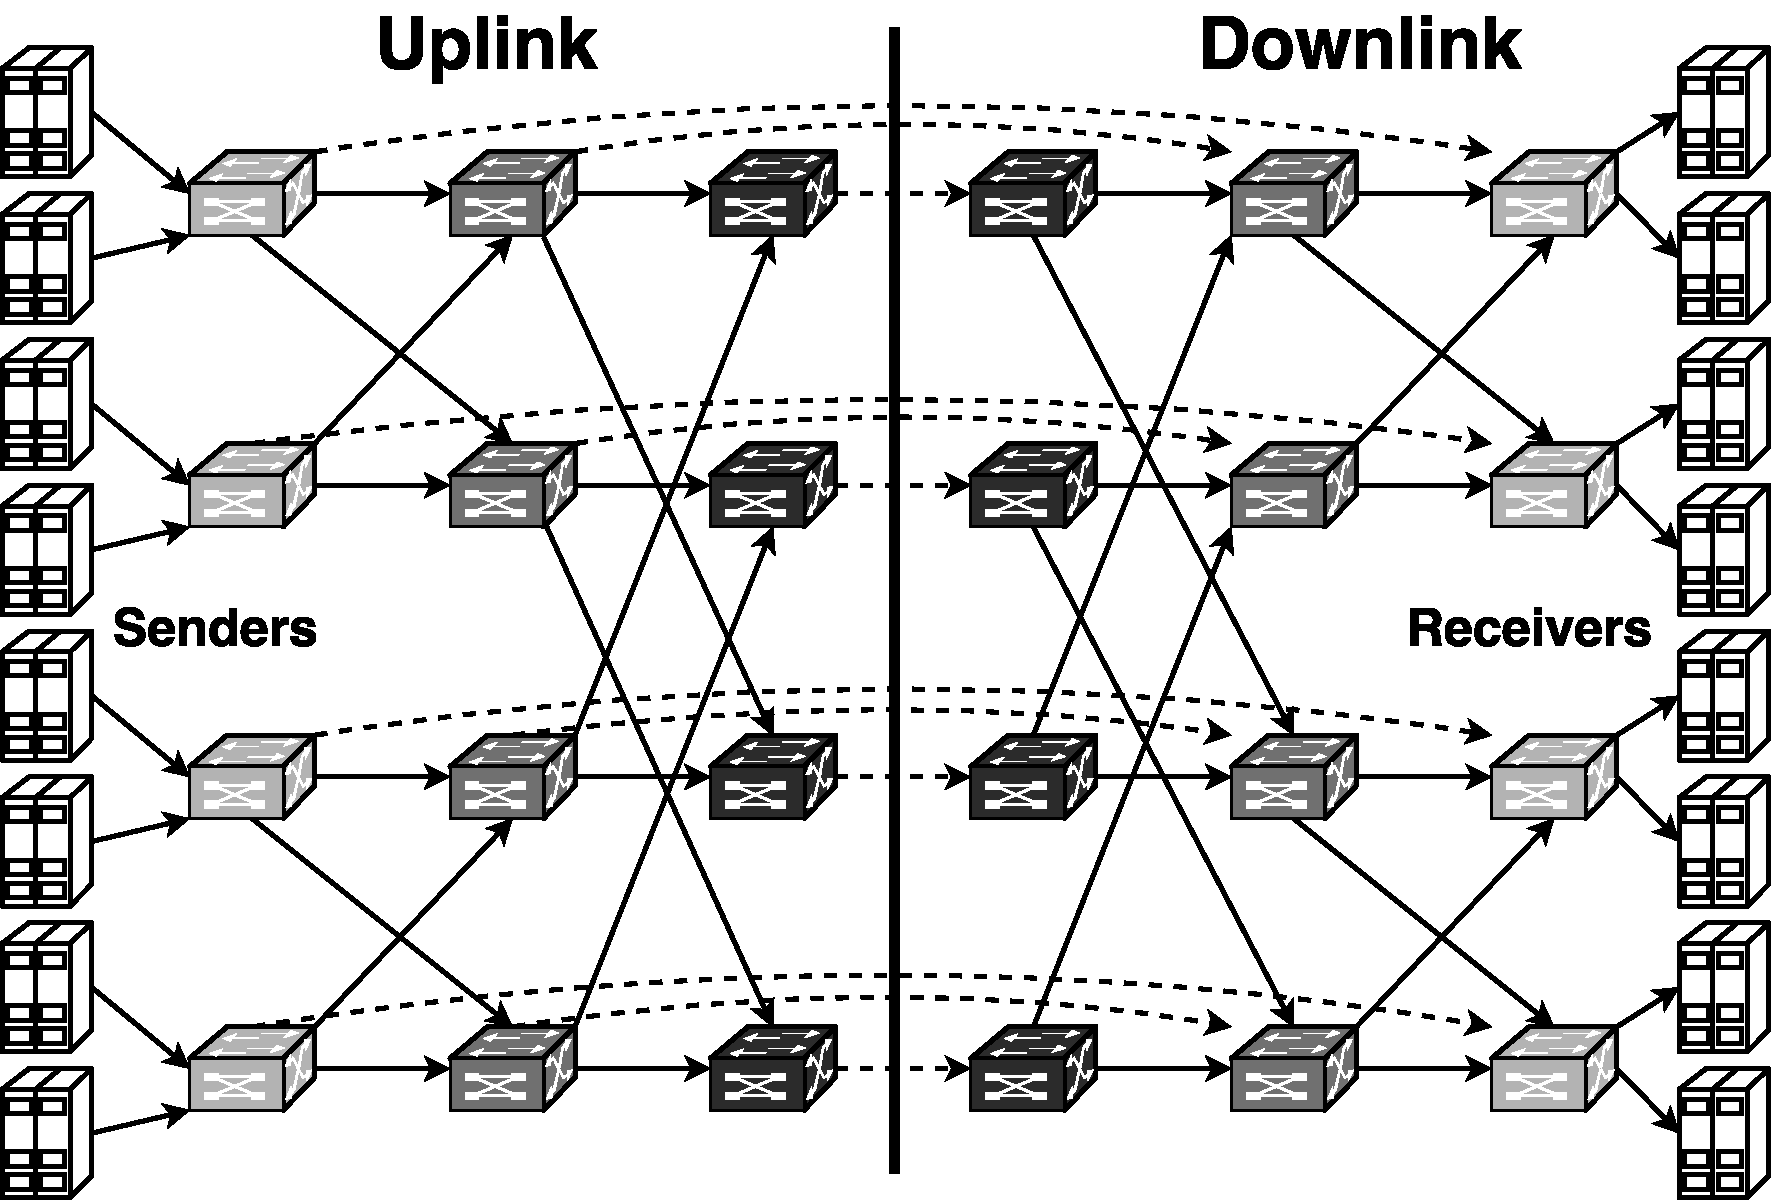
\includegraphics[width=.45\textwidth]{images/dcn_dag.pdf}}
%	\caption{Architecture of a typical data center network.}
%	\label{fig:dcn}
%\end{figure*}


\begin{figure}[t]
\centering
{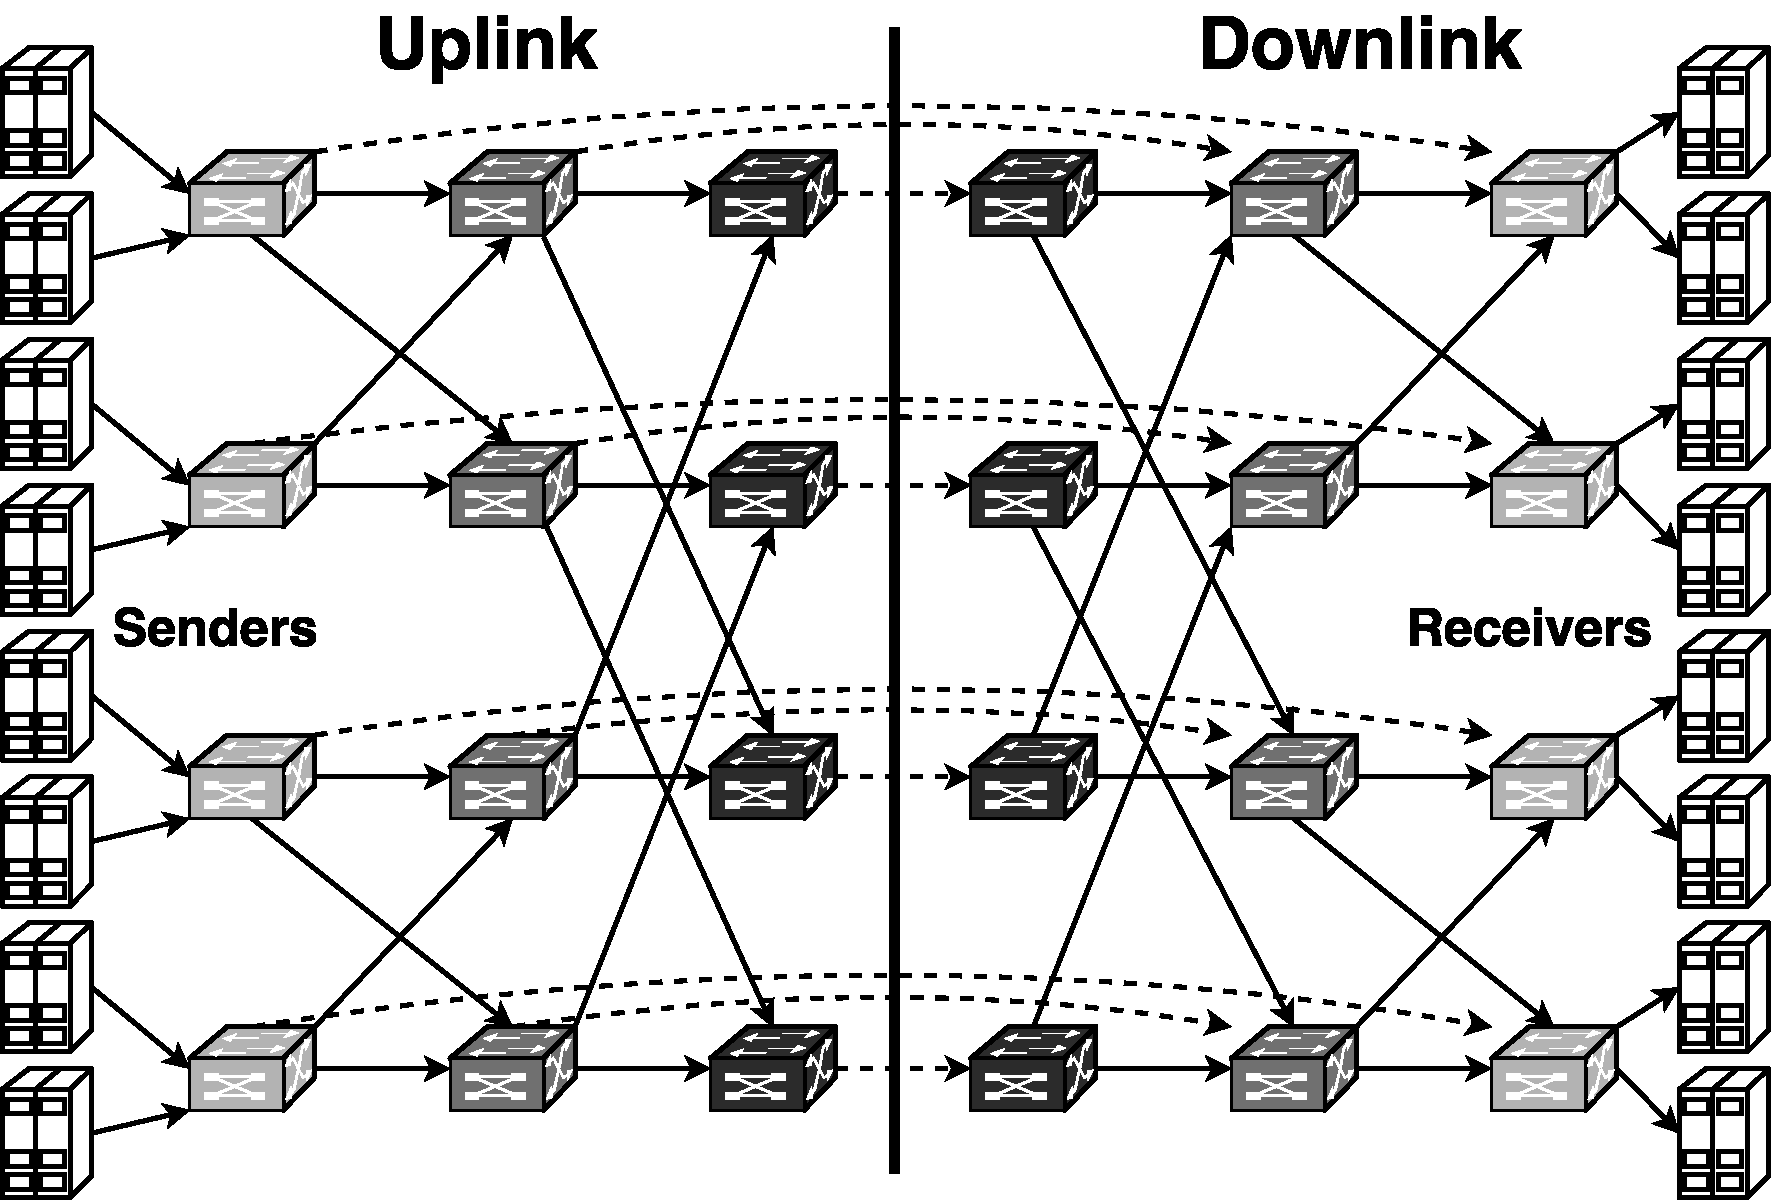
\includegraphics[width=.48\textwidth]{images/dcn_dag.pdf}}
\vspace{-20pt}
\caption{
	Routing topology of a typical data center network.
	Each physical switch is split into two logical switches, one for \textit{uplink} and one for \textit{downlink}.
    The dashed virtual link between corresponding uplink and downlink switch indicates ``loopback'' traffic from a lower-layer switch or host to another one.
}
\label{fig:dcn}
\vspace{-1em}
\end{figure}

\begin{figure}[t]
\centering
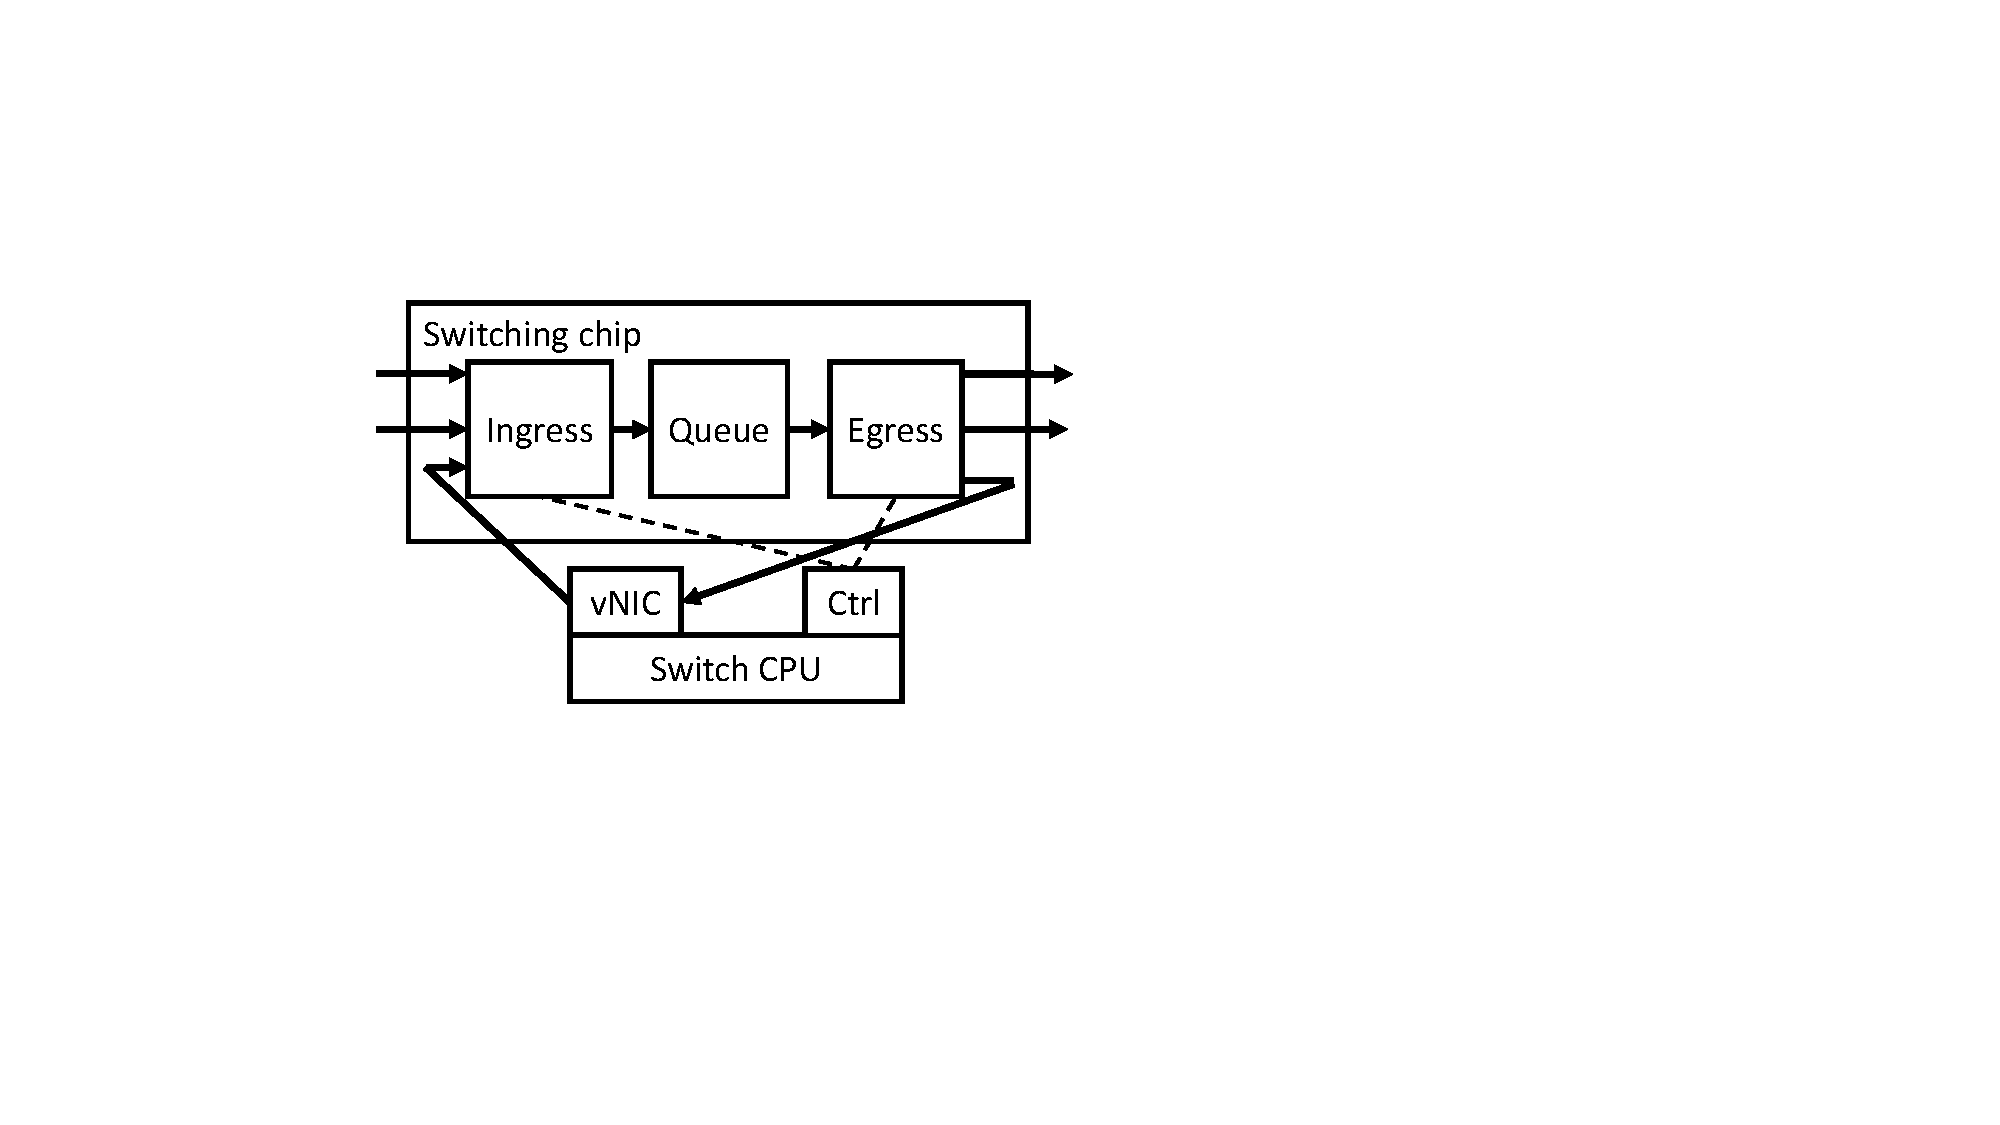
\includegraphics[width=0.3\textwidth]{images/cropped_switch_architecture.pdf}
\vspace{-10pt}
\caption{Architecture of a typical network switch.}
\label{fig:switch}
\vspace{-15pt}
\end{figure}

Modern data centers typically adopt multi-rooted tree topologies~\cite{leiserson1985fat,greenberg2009vl2} to interconnect hundreds of thousands of hosts. In a multi-rooted tree topology, the shortest path between two hosts first goes up to one of the lowest common ancestor switches, then goes down to the destination.
%Shortest-path between two hosts in a multi-rooted tree first goes up layers of switches to one of their lowest common ancestors, then goes down layers of switches.
Therefore, the routing topology form a directed acyclic graph (DAG), as shown in Figure~\ref{fig:dcn}.
This loop-free topology enables hierarchical aggregation of barrier timestamps.

Apart from the production network, data centers have an isolated management network that interconnects network switches.
A highly available SDN \emph{controller} runs on the management network to detect failures of switches and links, then reconfigure routing tables on failure.

%\RED{Discuss loop-free routing.}
%Formally, for $n$ distinct switches $S_1, \ldots, S_n$, if there are $n$ links $L_1, \ldots, L_n$ directly connecting $S_1 \rightarrow S_2, \ldots, S_{n-1} \rightarrow S_n, S_n \rightarrow S_1$, and $n$ possible routes (need not be distinct) passing through $L_1 \rightarrow L_2, \ldots, L_{n-1} \rightarrow L_n, L_n \rightarrow L_1$ respectively, then we call it a \textit{routing loop}.
%Loop-free is a liveness requirement.
%A routing loop stalls the update of timestamp barriers, but does not violate correctness.

\subsection{Programmable Switches}
\label{sec:programmable-switches}
The switch consists of a switching chip~\cite{broadcom,tofino} and a CPU (Figure~\ref{fig:switch}). The switch operating system~\cite{arista-eos} runs on the CPU to control the switching chip (\textit{e.g.} configure chip registers). The switching chip forwards selected traffic (typically control plane traffic, \textit{e.g.}, DHCP and BGP) to the CPU for processing via a virtual NIC. 

The switching chip is composed of an ingress pipeline, multiple FIFO queues and an egress pipeline.
When a packet is received from an \textit{input link}, it first goes through the ingress pipeline to determine the output link and queueing priority, then get buffered into the corresponding FIFO queue.
The egress pipeline pulls packets from queues according to priority, applies header modifications and sends them to \textit{output links}.
One key property of the switch is that the queuing model ensures \emph{FIFO} property for packets with the same ingress and egress port, 
if the packets have the same priority. In addition, packet corruption on input links and buffer overflow inside switches can be detected, and a packet loss counter is incremented per lost packet.

The data center switch can provide good programmability. First, the CPU can be used to process (a small amount of) data plane packets~\cite{lu2011serverswitch}.
Second, the switching chip is becoming more and more reconfigurable in recent years. For example, Tofino chip from Barefoot networks~\cite{tofino} 
%uses RMT architecture~\cite{bosshart2013forwarding} with 
supports flexible packet parsers, reconfigurable pipelines and stateful memory. Users can program Tofino using P4~\cite{bosshart2014p4} to achieve \textit{customized per-packet processing}.

Despite good programmability, the data center switch typically has limited buffer resource.
The average per-port on-chip buffer is typically hundreds of kilobytes~\cite{bai2017congestion} in size.
%Furthermore, the buffer size per port per Gbps keeps decreasing with the increase of link speed.
As a result, it is challenging to buffer many packets at the switches in a data center.


%, controls the switching chip and communicates with other switches via a management network. 

%There is a CPU port on the switching chip and a virtual NIC on the CPU to transfer control-plane packets (\textit{e.g.} DHCP, BGP) between the chip and the CPU. 


%Logically, the switching chip is composed of an \textit{ingress} pipeline, multiple queues and an \textit{egress} pipeline.
%Both ingress and egress pipelines are a chain of match-action tables. Each table can accomodate a number of rules. Each rule matches a set of packet header fields and internal states, and applies a limited repertoire of actions corresponding to common processing behaviors.
%When a packet is received from an input link, it first goes through the ingress pipeline (including tunnel decapsulation, routing, ACL rules and others) to determine the output link and queueing priority, then get buffered into the tail of the queue of corresponding priority. The egress pipeline pulls packets from the head of each queue according to scheduling disciplines, applies header modifications and sends them to the output links. This queueing model ensures FIFO property for packets with same priority.

%One limitation of most widely-deployed switching chips is the limited programmability of internal states that are persistent across packets. The Barefoot Tofino switching chip~\cite{tofino} using RMT architecture~\cite{bosshart2013forwarding} supports \textit{stateful per-packet processing} and has high programmability with P4~\cite{bosshart2014p4} language.
%However, the number of persistent states supported by each switch is only sufficient to have several per-port registers, but not enough to maintain per-packet states. 
%Furthermore, the buffer size of network switches is less than 1~MB per port~\cite{bai2017congestion}.
%Therefore, it is hard to implement a strict priority queue large enough for in-network serialization~\cite{sivaraman2016programmable}.

%\subsection{In-Network Computation}
%\label{sec:in-network}

%In-network computation flourishes with the trend of programmable switches (cite P4, Domino, serverswitch) and NICs (cite ClickNP, flexnic, VFP), opening up two categories of opportunities to distributed systems:

%\textit{Increase knowledge and control in network transmission.}
%In modern datacenters, there are multiple paths from a sender to a receiver for load balancing and fault tolerance. 
%Software-defined networking (SDN) enables visibility to routing table changes from BGP or administrators. In our scenario, in order to know the set of all possible input links per output link, \sys software on the affected switches need to be notified prior to route change.

%\textit{Offload computation on end hosts to reduce network traffic and latency.}
%\textit{Multicast} is an in-network computation to reduce duplication of messages on sender side.
%\textit{On-switch cache} is also a type of in-network computation to save computation on end hosts and improve load balancing (cite switchKV).
%A single network switch is a serialization point where \textit{coordination} of directly-connected hosts can take place (cite hardware coordination, Eris).
%\sys leverages the broadcast, cache and coordination functionalities of network switches to scale total ordering hierarchically.\RED{(leverage broadcast and cache?)}

%\textbf{Consider NIC as a switch, processes connect to data center network via NIC.}

\iffalse
\subsection{Network Requirements}
\label{sec:assumptions}

\sys assumes that the underlying network satisfies three properties, two for correctness and one for liveness.

\textbf{At-most-once Transport.}
The underlying transport of \sys should provide at-most-once semantics, \textit{i.e.}, each packet is transmitted at most once.
Otherwise, the retransmitted packet may violate timestamp ordering on the network link.
UDP or unreliable datagram in RDMA satisfies this requirement.

\textbf{FIFO on a Network Switch.}
If packets $P_1, P_2$ arrive in order to an input link of switch $S$, and they are routed to the same output link, then their output ordering should also be $P_1, P_2$.
In practice, packets from the same application typically have the same priority, so packet ordering is preserved after passing through a single switch.

\textbf{Loop-Free Routing.}
%Formally, for a switch $S$, its output links $E$ and input links $I$, if there is a possible route from an input link $i \in I$ to an output link $e \in E$, then add $i$ to the \textit{ingress set} of $e$.
Formally, for $n$ distinct switches $S_1, \ldots, S_n$, if there are $n$ links $L_1, \ldots, L_n$ directly connecting $S_1 \rightarrow S_2, \ldots, S_{n-1} \rightarrow S_n, S_n \rightarrow S_1$, and $n$ possible routes (need not be distinct) passing through $L_1 \rightarrow L_2, \ldots, L_{n-1} \rightarrow L_n, L_n \rightarrow L_1$ respectively, then we call it a \textit{routing loop}.
Loop-free is a liveness requirement.
A routing loop stalls the update of timestamp barriers, but does not violate correctness.
%Sec.~\ref{sec:eval-changes} evaluates temporary routing loops.
%Shortest-path (ECMP) routing in a Clos network is loop-free, which is common in datacenters.
%Shortest-path routing in a triangle is also loop-free. However, shortest-path routing in a pentagon is not loop-free, because the 5 routes $S_1 \rightarrow S_2 \rightarrow S_3, \ldots, S_5 \rightarrow S_1 \rightarrow S_2$ form a routing loop by our definition.
\fi
